%!TEX encoding = UTF-8
\documentclass[uplatex]{jsarticle}
\usepackage[dvipdfmx]{graphicx, color}
\usepackage{bmpsize}
\usepackage{wrapfig}
\usepackage{url}

\title{情報特論}
\author{32番 松川侑生}
\date{2020年 3月1日}

\begin{document}
\maketitle
\section{目的}
    Tello EDUの単眼カメラとDlibの顔検出を利用して顔追跡をおこなう。
\section{開発環境}
    \textit{Tello EDUの公式サイト}~\cite{tello}より、本体情報を表\ref{tab:tello}に示す。
\begin{table}[htbp]
  \centering
  \caption{Tello EDU 仕様概略}
  \begin{tabular}{lllll}  \hline
  重さ     & $87  $ g            \\ 
  大きさ    & $98 \times 92.5 \times 41 $ mm   \\ 
  最高速度   & $ 17.8$ mph   \\ 
  Wi-Fi  & 802.11n 2.4 GHz \\
  最長飛行時間 & $13$ min  \\ \hline
  \end{tabular}
  \label{tab:tello}
\end{table}

    ノートパソコン\\
\begin{table}[htbp]
  \centering
  \caption{ノートPC}
  \begin{tabular}{lllll}  \hline
  CPU     & Intel(R) Core(TM) i7-8565U $1.8$GHz    \\ 
  メモリ & $16$ GB   \\ 
  SSD & $256$ GB \\ \hline
  \end{tabular} 
  \label{tab:laptop}
\end{table}
\section{設計仕様}
システムシーケンスを図\ref{fig:sequence}に示す。ドローンから映像から送られてくる
映像をフレーム毎にDlibの顔認識を通し、顔と判定された矩形中心が画像の
位置によって制御命令を送る。また、距離はドローンの表示領域面積が一定になるように
制御命令を送る。
\begin{figure}[]
    \centering
    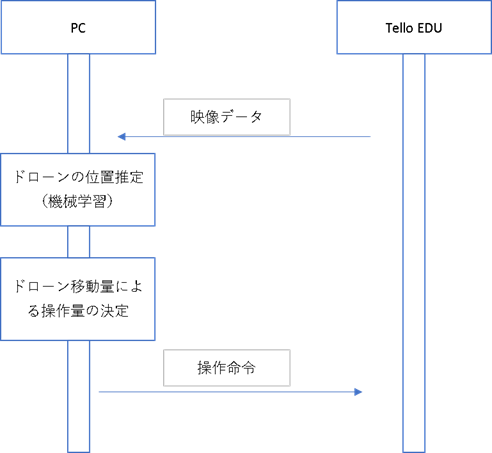
\includegraphics{sequence.png}
    \caption{システムシーケンス}
    \label{fig:sequence}
\end{figure}  
\section{開発結果}
本システムは低速度下でのみ動作することが確認できた。また、十分な光量と顔正面から
の映像が不可欠である。
\section{考察}
さらなるシステムの改善には横顔の認識や口頭部の認識も必要だと考えられる。一例として、
3Dモデルの認識ができないか検討するのもいいだろう。

\bibliographystyle{jplain}
\bibliography{refer}

\end{document}